\documentclass[../main.tex]{subfiles}
\begin{document}

\chapter{Seminal work: TWAS from individual-level data}
\labch{gamazon2015}

\begin{external_abstract}{title=Abstract}
Genome-wide association studies (GWAS) have identified thousands of 
variants robustly associated with complex traits. However, the 
biological mechanisms underlying these associations are, in general, not 
well understood. We propose a gene-based association method called 
PrediXcan that directly tests the molecular mechanisms through which 
genetic variation affects phenotype. The approach estimates the 
component of gene expression determined by an individual's genetic 
profile and correlates 'imputed' gene expression with the phenotype 
under investigation to identify genes involved in the etiology of the 
phenotype. Genetically regulated gene expression is estimated using 
whole-genome tissue-dependent prediction models trained with reference 
transcriptome data sets. PrediXcan enjoys the benefits of gene-based 
approaches such as reduced multiple-testing burden and a principled 
approach to the design of follow-up experiments. Our results demonstrate 
that PrediXcan can detect known and new genes associated with disease 
traits and provide insights into the mechanism of these associations.
\end{external_abstract}

\section{Introduction}

Albeit it is accepted that in the majority of cases the biological role 
of variants associated to diseases is regulatory, as confirmed by the 
fact that many such variants fall in regions that are epigenetically 
marked as regulatory, GWAS results remain mainly uncharacterised from a 
functional point of view, and are only able to explain a little 
proportion of phenotypic variance. The wealth of biological data that is 
now being released by large-scale consortia provides an unprecedented 
opportunity to integrate information and obtain insight into the genetic 
and biological processes underlying disease susceptibility\sidenote{Some 
of these consortia, whose data sets have been used by Gamazon \etal, are 
the following.
\begin{description}
	\item[ENCODE.] The focus is on the systematic functional annotation 
of each segment of the human genome.
	\item[GEUVADIS.] This project endeavours to uncover functional 
variation in humans through the study of how genetic variants affect 
gene expression.
	\item[DGN.] Variants regulating gene expression, splicing and 
allelic expression are detected.
	\item[Braineac.] The authors find eQTL in ten human brain regions.
	\item[GTEx Project.] Its aim is to collect data on genotype and gene 
expression levels of a number of tissues from postmortem samples.
\end{description}
}.

This work is based on two key ideas: first, genetic variants most often 
impact gene expression, as shown by the many eQTL studies; second, SNP 
aggregation methods that combine many variants in a biologically 
meaningful way have the potential to improve GWAS results. Therefore, 
the authors propose to group together all the SNPs that regulate the 
expression of a given gene. One advantage of this approach, which they 
called PrediXcan, is that statistical tests performed on group of SNPs 
are more powerful than those performed on each and every SNP due to less 
multiple testing; besides, by choosing the gene as a grouping unit, 
information about the directionality of the effect is intrinsically 
provided, \ie it is possible to say whether the disease is associated to 
an increase or a decrease in the gene's expression. Moreover, from a 
functional point of view a gene is much more interpretable than a simple 
genetic polymorphism.

\section{Method}

The main goal is to provide a framework to better interpret GWAS 
results. However, in a typical GWA study the individuals are simply 
genotyped with a SNP microarray, and expression data are completely 
missing. Therefore, gene expression has to be predicted by exploiting 
the knowledge of expression quantitative trait loci.

The first assumption here is that gene expression can be decomposed into 
three components: genetically regulated expression (GReX), 
phenotype-influenced expression, and an environment-determined component 
(\reffig{gamazon2015/1}). Some phenotype, such as many diseases, can 
indeed influence gene expression, but, as we shall see in a moment, by 
training their predictive models on healthy individuals from reference 
transcriptome experiments, they already exclude that component from what 
they predict.

\begin{figure}
	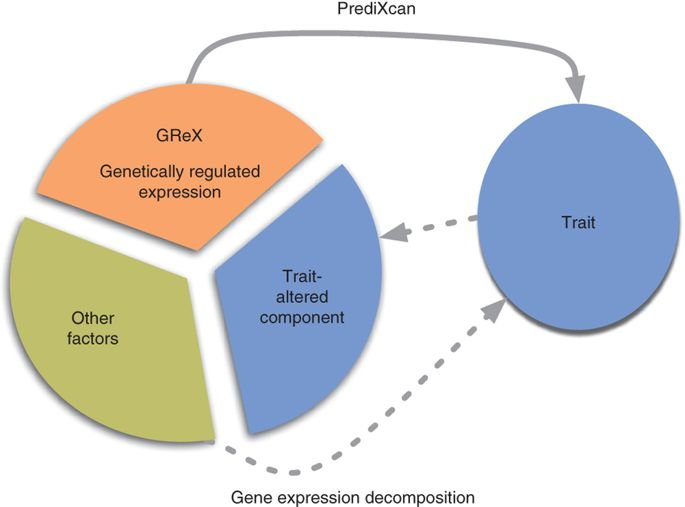
\includegraphics{gamazon2015/1-expression_decomposition}
	\caption{Gene expression can be decomposed into three components}
	\labfig{gamazon2015/1}
\end{figure}

The prediction relies on data sets where both genotype and expression 
are present, such as the aforementioned GEUVADIS and GTEx projects, and 
the model is additive (\reffig{additive_model}), meaning that a given 
variant in a homozygous individual is supposed to have twice the effect 
of that same variant in an heterozygous individual. This is surely an 
oversimplification, for it does not take into account three biologically 
important effects ---epistasis, dominance and penetrance---, but an 
additive model is much simpler to implement. The purpose of this 
regression model, which is an elastic net (see \refsec{regression} 
Regression) with $\alpha = 0.5$, is to find for each SNP the coefficient 
of which gene expression is altered by a copy of that SNP. Once the 
coefficients have been estimated, the genetically regulated component of 
gene expression can be predicted starting only from the genotype of an 
individual; the predicted GReX is denoted as $\hat{GReX}$.

\begin{marginfigure}{-1cm}
	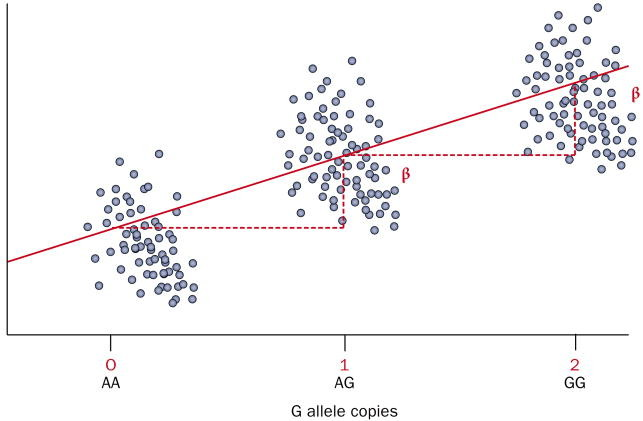
\includegraphics{gamazon2015/ext-additive_genetic_model}
	\labfig{additive_model}
	\caption{An example of additive model for one SNP; Gamazon \etal 
extended it for several SNPs. Image adapted from Conall M. O'Seaghdha 
and Caroline S. Fox, \enquote{Genome-wide association studies of chronic 
kidney disease: what have we learned?}}
\end{marginfigure}

\enquote{(For specific results on the disease phenotypes analyzed here, 
we used logistic regression with disease status.)} by fmarotta: they 
used a binary variable, but what about using the liability to the 
disease, which is continuous? see visscher 2008.

\begin{equation}
	T = \sum_{k=1}^{M}{w_k X_k + \epsilon}
\end{equation}

T is the expression of a gene, $w_k$ is the weigth of SNP k in influencing the
expression of that gene, and $X_k$ is the number of reference alleles of SNP k
(I guess $X_k$ is the sum of the alleles in all the individuals in the
dataset).

consideration by fmarotta: there are other models available, for instance one
could account for the penetrance, or use a dominant (recessive) model, and so
on.

Important (by fmarotta): in linear regression, each regressor is considered
independent of the others, but is that so? I think often a phenotype can depend
on the \textit{combination} of SNPs.

(also by fmarotta): is it possible to use PCA to find which SNPs are most
relevant in influencing a phenotype?

In the second phase, the predicted GReX is correlated (with linear regression,
logistic regression, Cox, or Spearman (the latter is non-parametric). They used
logistic regression for the results discussed in this article.

limits: there is an attenuation bias because of the error in the estimation of
the GReX.

\section{features}

The rationale for everything is that often SNPs influence a phenotype by
altering gene expression (\ie they have regulatory roles), as stated in 
this
article:
http://journals.plos.org/plosgenetics/article?id=10.1371/journal.pgen.1000888

main advantages:

\begin{itemize}
\item directionality, possibility to get insights on mechanisms.
\item small multiple-testing burden.
\item possibility form functional units (e.g. basing on known pathways).
\item possibility to reanalise gwas data (only the genome is needed).
\end{itemize}

%\section{Prereq: 
%https://www.sciencedirect.com/science/article/pii/S0002929710005987?via%3Dihub}

%\subsection{pre-prereq: https://www.nature.com/articles/nature08494}



\section{Predicting the transcriptome}

They tried lasso, elastic net and another thing which turned out to be 
pretty bad and was abandoned. Lasso is a regression analysis whereby the 
number of regressors is diminished: some covariates are disregarded 
(their coefficient becomes 0), and in general only one covariate is 
selected from a set of highly correlated covariates. This is achieved by 
imposing the constraint that the sum of all the coefficients (in 
absolute value) must be less than a fixed amount $t$ (see wikipedia). 
Lasso explores a different path from ridge regression, where the sum of 
the squares of the coefficients must be less than an amount. Elastic net 
is an improvement of lasso, where an additional constraint is imposed: 
the linear combination of lasso and ridge constraints. The relative 
weight of the two constraints is moduled by the alpha coefficient: the 
linear combination is alpha*L1 + (1-alpha)*L2.

In general lasso (elastic net) is used 1) because the number of 
predictors is HUGE, especially if compared to the number of samples; 2) 
to avoid overfitting.

They chose to use elastic net and used tenfold cross-validation (\ie 
they looked at the R square of estimated GReX vs observed expression).

They also computed the heritability of gene expression in DGN and claim 
that heritability \marginnote{Heritability is defined as the proportion 
of phenotypic variance that is due to genetic variance} is an upper 
bound to how well the trait can be associated to the genotype. This 
makes sense, because if the variance in a trait is entirely due to the 
environment, the association study will not find anything.

The average heritability calculated in DGN was 0.153, while the average 
tenfold cross-validated prediction $R^2$ value for elastic net was 
0.137, so: not bad. Does this make sense? I think so, because 
  heritability can be interpreted as the slope of the line of the 
predicted variable as a function of the predictor (\eg offspring height 
as a function of parent height). In this case the "predictor" is the 
phenotype of the training sample, and the "predicted" is the phenotype 
in the testing sample. A high heritability says that parent height can 
predict offspring height, and that this predictability is due to genetic 
factors; here, the authors are trying to predict a phenotype (gene 
expression, but it is hardly relevant) from a genotype, which in turn 
was attributed scores according to the phenotype. The linear model 
(actually elastic net) they made, mimics the actual process of 
development: they go from one genotype to a phenotype, attributing to 
each element of the genotype (\ie to each SNP) a coefficient that 
measures how much that element is involved in the manifestation of that 
phenotype. Then, let us imagine that the training people have offspring, 
and that the offspring is the "testing people": many of the SNPs will be 
transmitted from parents to offspring. offspring have a similar genotype 
to their parents (abstracting things, offspring are merely people which 
have a genome similar to their parents), but do they have also a similar 
phenotype? If the trait is heritable, yes. In yet other words, if the 
trait is heritable, people with a similar genotype (\ie relatives) will 
have a similar phenotype (h2 is precisely the correlation between the 
phenotypes in parents-offspring); in a sense, in this paper the testing 
people (those in the gwas) are relatives of the training people (those 
in the reference transcriptome study like GEUVADIS). All this is 
expressed in figure 3.

An important thing that perhaps I did not say before is that previously 
they had imputed the SNPs of the DGN people. They used both 1000 Genomes 
and HapMap Phase 2 to impute, and achieved similar results, therefore 
they chose to restrict the imputation to hapmap to save computation 
time.

They then tested their models to see wether, given a genotype, they 
could predict the expression. That is to say, they predicted expression 
from a set of genotypes and then confronted it with the real expression. 
They used GEUVADIS and GTEx as tests. In figure 4 they show that the 
correlation between predicted and actual expression in this separate 
cohort is very different from the expected correlation under the 
hypothesis that the two vectors (predicted and actual expression) are 
independent. In gray there is a 45-degree line: if the point lay on this 
line, then on the two axes there are identical variables. on the y axis 
there are the quantiles of observed R2 (a quantile is the percentage of 
points below a given value), while on the x axis there are the quantiles 
of expected R2. A point is produced when the two quantiles are equal. 
For instance, if the 10th quantile in the observed R squareds have an R2 
of 0.2, what is the R2 of the expected R2 at the 10th quantile? In other 
words, the curve is parametric. This Q-Q plot is used to check whether 
two populations are similar.

They also note that the same situation arises for different tissues.

In fig 5 they present some example genes.

they also made a linear model for trans eQTL, with linear regression, 
but it had a poorer predictive power, so they resolved to use local SNPs 
only.

\section{Application of PrediXcan to WTCCC}

At last, they apply their method. they used DGN whole-blod elastic net 
prediction models to predict the expression in the WTCCC cohort, then 
correlated the predicted GReX with the disease status.

An interesting consideration (by fmarotta) is that many of the genes 
that were associated to the disease status were in the HLA or MHC 
region; also, the most significant results were for autoimmune diseases 
(this can be due to the fact that also in the WTCCC work the most 
significant results were for autoimmune diseases. Nay, I think that the 
fact that the two studies (WTCCC and gamazon) have found the same result 
is due to a common underlying cause, which is the same for which most 
GWAS hits are in the MHC region.) Think more about this.

They made a manhattan plot and another quantile-quantile plot. Also a 
gwas enrichment.

Some genes were associated with multiple autoimmune disease. Question by 
fmarotta: what determines which disease you have if the expression of 
that gene is altered in you? environment? gene expression level? Anyway, 
this is an example of the complexity of the situation: the relationship 
between genotype and phenotype is not biunivocal at all. the authors say 
that lower expression of dclre1b was associated with rheumatoid 
arthritis and T1D, whereas higher expression with crohn's disease.

An advantage of predicscan is that it provides directionality: we know 
if higher or lower expression is associated with the disease. See the 
example of ERBB3.

Globally, many genes were previously reported or fell near reported 
genes. Or: they were in the MHC.

Using less stringent significance thresholds, they found the same high 
enrichments of reported genes among the results of predicscan. This 
suggests that there are many false-negatives at the higher thresholds. 
The method is not so powerful afterall. They found also two completely 
novel genes.

Finally, they compared their method with two other gene-based tests: 
vegas and skat. In the quantile-quantile plot, predixcan was the best in 
the tail-end.

\section{Discussion}

Why gene expression? It is the most direct phenotype (indeed, sometimes 
we speak about \enquote{extended phenotypes}; gene expression can also 
be viewed as an intermediate phenotype), it is heritable, and virtually 
all the other phenotypes depend on it. Moreover, it is easy to measure.

fmarotta:Genes can do few things: either they bind proteins whith a 
structural or regulatory function (and when it is structural, it can be 
regulating: TAD are coregulated), or they are transcribed, starting a 
series of biochemical reactions that ultimately lead to functional 
molecules, be they RNA or proteins. The complexity stems from the 
interactions of many genes together and with the environment

Limits:
\begin{itemize}
	\item
the prediction of gene expression can be biased, and some models, namely 
a combination of K nearest neighbour (KNN), elastic net, and the use of 
genomic annotation may perform better.
	\item 
(https://www.cell.com/ajhg/fulltext/S0002-9297(18)30108-3?code=cell-site) 
Genetic variation does not alter only gene expression. There can be 
\textit{trans}-acting effects, where a SNP alters how a gene (be it a TF 
or a miRNA) modulates the expression of others, without altering the 
expression of the modulator gene itself. Moreover, a SNP can have 
effects on splicing, transcription start or end site or other RNA 
editing processes, without altering the expression of the gene.
\end{itemize}

One of the main advantages is that it is economic: one only needs 
existing data, therefore many existing GWAS dataset can be reanalysed 
\enquote{for free}.

Another virtue is that predicscan provides directionality, hinting at 
potential strategies to cure disease, \eg if a gene's upregulation is 
linked to a disease, then a drug may be developed to downregulate it. 
(by fmarotta: It probably woul have no effect whatsoever because of 
compensatory effects.)

Multiple testing: here they have used bonferroni, which is pretty 
conservative. They only corrected gene-based tests of association, and 
not SNP-based ones, because the gene-based association is the last step, 
and because bonferroni is conservative. (by SNP-based, I do not know if 
they mean SNP-geneexpression association or SNP-trait association 
performed in a classical GWAS.)

They do not claim causality, for SNPs may contribute both to expression 
and to other things, and it may be that the other things are the cause 
of the disease, not gene expression.

They state that their method provides insights into gene regulation and 
directionality.

by fmarotta: Actually, they do not prove that a SNP associated to gene 
expression regulates the gene: they  only say that variation between 
individuals at that locus results in variation in gene expression. Or do 
they?

\end{document}
